% Options for packages loaded elsewhere
\PassOptionsToPackage{unicode}{hyperref}
\PassOptionsToPackage{hyphens}{url}
%
\documentclass[
]{article}
\usepackage{amsmath,amssymb}
\usepackage{lmodern}
\usepackage{ifxetex,ifluatex}
\ifnum 0\ifxetex 1\fi\ifluatex 1\fi=0 % if pdftex
  \usepackage[T1]{fontenc}
  \usepackage[utf8]{inputenc}
  \usepackage{textcomp} % provide euro and other symbols
\else % if luatex or xetex
  \usepackage{unicode-math}
  \defaultfontfeatures{Scale=MatchLowercase}
  \defaultfontfeatures[\rmfamily]{Ligatures=TeX,Scale=1}
\fi
% Use upquote if available, for straight quotes in verbatim environments
\IfFileExists{upquote.sty}{\usepackage{upquote}}{}
\IfFileExists{microtype.sty}{% use microtype if available
  \usepackage[]{microtype}
  \UseMicrotypeSet[protrusion]{basicmath} % disable protrusion for tt fonts
}{}
\makeatletter
\@ifundefined{KOMAClassName}{% if non-KOMA class
  \IfFileExists{parskip.sty}{%
    \usepackage{parskip}
  }{% else
    \setlength{\parindent}{0pt}
    \setlength{\parskip}{6pt plus 2pt minus 1pt}}
}{% if KOMA class
  \KOMAoptions{parskip=half}}
\makeatother
\usepackage{xcolor}
\IfFileExists{xurl.sty}{\usepackage{xurl}}{} % add URL line breaks if available
\IfFileExists{bookmark.sty}{\usepackage{bookmark}}{\usepackage{hyperref}}
\hypersetup{
  pdftitle={Final Project: Predicting Cervical Spine Injuries in Children},
  pdfauthor={Andy Shen, Licong Lin, Seunghoon Paik},
  hidelinks,
  pdfcreator={LaTeX via pandoc}}
\urlstyle{same} % disable monospaced font for URLs
\usepackage[margin=1in]{geometry}
\usepackage{graphicx}
\makeatletter
\def\maxwidth{\ifdim\Gin@nat@width>\linewidth\linewidth\else\Gin@nat@width\fi}
\def\maxheight{\ifdim\Gin@nat@height>\textheight\textheight\else\Gin@nat@height\fi}
\makeatother
% Scale images if necessary, so that they will not overflow the page
% margins by default, and it is still possible to overwrite the defaults
% using explicit options in \includegraphics[width, height, ...]{}
\setkeys{Gin}{width=\maxwidth,height=\maxheight,keepaspectratio}
% Set default figure placement to htbp
\makeatletter
\def\fps@figure{htbp}
\makeatother
\setlength{\emergencystretch}{3em} % prevent overfull lines
\providecommand{\tightlist}{%
  \setlength{\itemsep}{0pt}\setlength{\parskip}{0pt}}
\setcounter{secnumdepth}{5}
\usepackage{float}
\usepackage{bbm}
\usepackage{graphicx}
\usepackage{array}
\usepackage{blindtext}
\usepackage{color}
\usepackage{subfloat}
\ifluatex
  \usepackage{selnolig}  % disable illegal ligatures
\fi
\newlength{\cslhangindent}
\setlength{\cslhangindent}{1.5em}
\newlength{\csllabelwidth}
\setlength{\csllabelwidth}{3em}
\newenvironment{CSLReferences}[2] % #1 hanging-ident, #2 entry spacing
 {% don't indent paragraphs
  \setlength{\parindent}{0pt}
  % turn on hanging indent if param 1 is 1
  \ifodd #1 \everypar{\setlength{\hangindent}{\cslhangindent}}\ignorespaces\fi
  % set entry spacing
  \ifnum #2 > 0
  \setlength{\parskip}{#2\baselineskip}
  \fi
 }%
 {}
\usepackage{calc}
\newcommand{\CSLBlock}[1]{#1\hfill\break}
\newcommand{\CSLLeftMargin}[1]{\parbox[t]{\csllabelwidth}{#1}}
\newcommand{\CSLRightInline}[1]{\parbox[t]{\linewidth - \csllabelwidth}{#1}\break}
\newcommand{\CSLIndent}[1]{\hspace{\cslhangindent}#1}

\title{Final Project: Predicting Cervical Spine Injuries in Children}
\usepackage{etoolbox}
\makeatletter
\providecommand{\subtitle}[1]{% add subtitle to \maketitle
  \apptocmd{\@title}{\par {\large #1 \par}}{}{}
}
\makeatother
\subtitle{Statistics 215A - Statistical Models: Theory and Application}
\author{Andy Shen, Licong Lin, Seunghoon Paik}
\date{\textbf{Acknowledgments:} Michael Boyle, Chandan Singh, Omer
Ronen, Bin Yu}

\begin{document}
\maketitle

\newcommand{\blue}{\textcolor{blue}}
\newcommand{\red}{\textcolor{red}}
\newcommand{\bb}{\textbf}

\hypertarget{introduction-and-domain-problem}{%
\section{Introduction and Domain
Problem}\label{introduction-and-domain-problem}}

Cervical spine injuries (CSI) include injuries sustained to the spinal
cord connecting the head and neck to the rest of the body. These
injuries, albeit rare, are extremely severe for children whose bodies
are still developing. CSI detection strategies include the use of a
\textbf{computed tomography (CT) scan}, among others. While these
interventions are generally effective at pinpointing injuries, they have
the potential to inadvertently expose children to ionizing radiation and
cause unnecessary pain (Leonard et al. (2011)).

The rarity of a CSI, in conjunction with the potentially harmful effects
of CSI detection methods, force clinicians and specialists to assess the
risk of performing a CT scan against the potential of missing critical
injury diagnoses. These judgement calls are typically supported through
a \textbf{clinical decision rule (CDR)} which uses prior data of CSI
injuries to predict whether a patient has sustained a true CSI or not.
Doctors use the results of the CDR and their own assessment of the
situation to decide if the risk of a CT scan outweighs its potential
benefits.
\textcolor{red}{Include more about how to IMPROVE the current CDR, most likely after we finish our model.}

In this project, we develop a CDR for predicting CSI in children, based
on data provided by the Pediatric Emergency Care Applied Research
Network (PECARN). The data are described in Section
\textcolor{blue}{\ref{sec:data}}. \textbf{Our objective is to predict
the true outcome of a patient's trauma (whether they truly have a CSI).}
We ensure all components of our CDR are interpretable and realistically
accessible to physicians when speculation of a CSI is called into
question. Throughout the modeling process, we ensure that our
predictions are accurate, stable, and capture the wide range of possible
injuries, as well as the varying medical and demographic history of each
patient.

The structure of this report is as follows: In Section
\textcolor{blue}{\ref{sec:data}}, we explain our data and the features
used to predict CSI. In\ldots{}

\hypertarget{sec:data}{%
\section{Data Collection}\label{sec:data}}

\textcolor{red}{The questions below are useful to ask: How were the data collected? At what locations? Over what time period? Who collected them? What instruments were used? Have the operators and instruments changed over the period? Try to imagine yourself at the data collection site physically.}

\textcolor{red}{INCLUDE NUMBER OF CONTROL AND CASE PATIENTS IN THE FINAL CLEANED DATA.}

As mentioned above, our data is collected from the PECARN hospital
network, which contains patient CSI data from a previous CDR study. The
previous study contained children both with and without CSI. The
children without CSI were grouped into various controls based on their
injury mechanism and whether they had received out-of-patient emergency
medical services (EMS) treatment.
\textcolor{red}{In our study, we are only interested in distinguishing true injury from simple trauma. We group all of the sub-control groups into a single control group for more refined predictions.}

The data consist of 12 datasets, each containing various categories of
information about the patients, such as demographics, medical history,
mechanism of injury, their appearance at the time of response and
arrival at the hospital, among others.

Some of the datasets have the same name, but are denoted with an
\texttt{field}, \texttt{out} or \texttt{site} at the end of the file
name (e.g \texttt{clinicalpresentationfield} vs
\texttt{clinicalpresentationsite}). The suffix ``field'' denotes
measurements of the patient at the location where the injury was
sustained, such as the site of the car crash or the patient's home. The
suffix ``out'' refers to information reported by an outside hospital
referring the patient to the PECARN system. Note that this information
is not available for patients who were not referred by an outside
hospital. The suffix ``site'' refers to information collected at the
PECARN hospital site. \textbf{The site information is always collected
last}, with the outside hospital information collected between field and
site if pertinent.

It is also important to recognize that this data is extremely prone to
human and/or machine error. We describe potential lapses in the data
collection process in Section \textcolor{blue}{\ref{sec:meaning}}. The
data cleaning process is discussed in Section
\textcolor{blue}{\ref{sec:clean}}.

\hypertarget{sec:meaning}{%
\subsection{Meaning}\label{sec:meaning}}

In order to better group the variables in our data, we separate them
into \textbf{three distinct categories: demographic information, injury
mechanism, and trauma presentation.} Demographic information simply
refers to the patient's basic information, such as age, gender, and
ethnicity. While these features may have very little predictive power,
they can be useful in grouping injured or non-injured patients post-hoc.

Injury mechanism refers to how the patient sustained their trauma.
Examples of injury mechanism include a vehicle accident, child abuse,
assault, or falling. Each category of injury is then further elucidated
into more specific modes of injury (such as a rear-end collision vs a
side impact collision). Most mechanisms of injury in the given data are
injuries sustained from various youth sports or from a motor vehicle
accident.
\textcolor{red}{Discuss later whether mechanism is actually useful or not}.

Finally, trauma presentation refers to the condition of the patient when
they arrive to the hospital or at the site of trauma. These features are
spanned across multiple datasets. Features in this category include
whether the patient is conscious or not, whether they report neck or
facial pain, whether their mental status appears to be normal, among
others.

Note here that some features across these three categories preclude
accurate reporting of others. For example, if a patient is unconscious
or cannot communicate properly, they will be unable to properly describe
whether they are in pain.

For our study, we prioritize using the ``site'' data if it is available,
imputing necessary missing values from outside hospital data and site
data in that order. We select the site data since it is most recent in
terms of a patient's trauma presentation. Features in the other two
categories do not differ across location and are named in an unsuffixed
dataset.

The non-demographic variables all measure some aspect of the patient's
trauma and allows us to assess how serious it is. Each piece of data was
recorded from multiple different perspectives. The measurements were
collected differently across 2-3 different locations and at 2-3
different time periods - the actual values could differ across time and
location. Moreover, the instruments used to take each measurement could
be calibrated differently or the individual taking the measurement could
have made a mistake. It is very important to keep these sources of error
in mind in the modeling process and when questioning unusual
observations.

By assuming our data is correct, we are assuming that\ldots{}

\textcolor{red}{What does each variable mean in the data? What does it measure? Does it measure what it is supposed to measure? How could things go wrong? What statistical assumptions is one making by assuming things didn’t go wrong? (Knowing the data collection process helps here.)}

\textcolor{red}{Meaning of each variable -- ask students to imagine being there at the ER and giving a Glasgow coma score, for example, and also a couple of variables -- ask students what could cause different values written down.}

\textcolor{red}{How were the data cleaned? By whom?}

\hypertarget{relevance}{%
\subsection{Relevance}\label{relevance}}

\textcolor{red}{Can the data collected answer the substantive question(s) in whole or in part? If not, what other data should one collect? The points made in (2) are pertinent here.}

The data provided are relevant to our study. The features described in
our model are all accessible to a physician when they make their
clinical decision. If any additional data is necessary, it could include
other potentially useful features that are typically made available to a
physician at the time of making the clinical decision. We do not collect
any more data since we are provided with all of the data recorded by
PECARN and it is highly unlikely that additional data with predictive
power exists.

\hypertarget{sec:eda}{%
\section{Exploratory Data Analysis}\label{sec:eda}}

\hypertarget{reducing-feature-space}{%
\subsection{Reducing feature space}\label{reducing-feature-space}}

Our initial feature space included over 300 features and an
interpretable model only requires a small fraction of these features. We
trim down our initial subset of features through the consultation of
domain experts in cervical spine injury. Utilizing the assistance of
Dr.~Michael Boyle, a physician in the UC San Francisco School of
Medicine, we reduced our feature space to roughly 51 variables to
perform variable selection on. The feature selection criteria is
discussed in Section \textcolor{blue}{\ref{sec:feat-sel}}.

The omitted features were mostly redundant information or information
that would not be provided to a physician when making a clinical
decision. These omissions were largely determined through domain-expert
judgment calls. When in doubt, we retained a predictor to avoid
potentially losing crucial predictive information. As discussed in
Section \textcolor{blue}{\ref{sec:feat-sel}}, we use a variable
selection process to determine our best features for modeling.

\hypertarget{sec:clean}{%
\subsection{Data Cleaning}\label{sec:clean}}

\hypertarget{correlation-heatmap}{%
\subsection{Correlation Heatmap}\label{correlation-heatmap}}

Figure \textcolor{blue}{\ref{fig:corr-map}} shows a heatmap of the
reduced feature space of 51 variables. While most features are not
strongly correlated with each other, there are some features that
exhibit high correlations. These features are typically those of the
same type, such as whether the patient reported pain in their neck and
whether tenderness was observed in the patient's neck. It is expected
for features like these to be influenced by one another. Moreover, most
features have absolute correlation \(|\rho| < 0.5\), indicating weak
association throughout the feature space in general.

\begin{figure}[H]
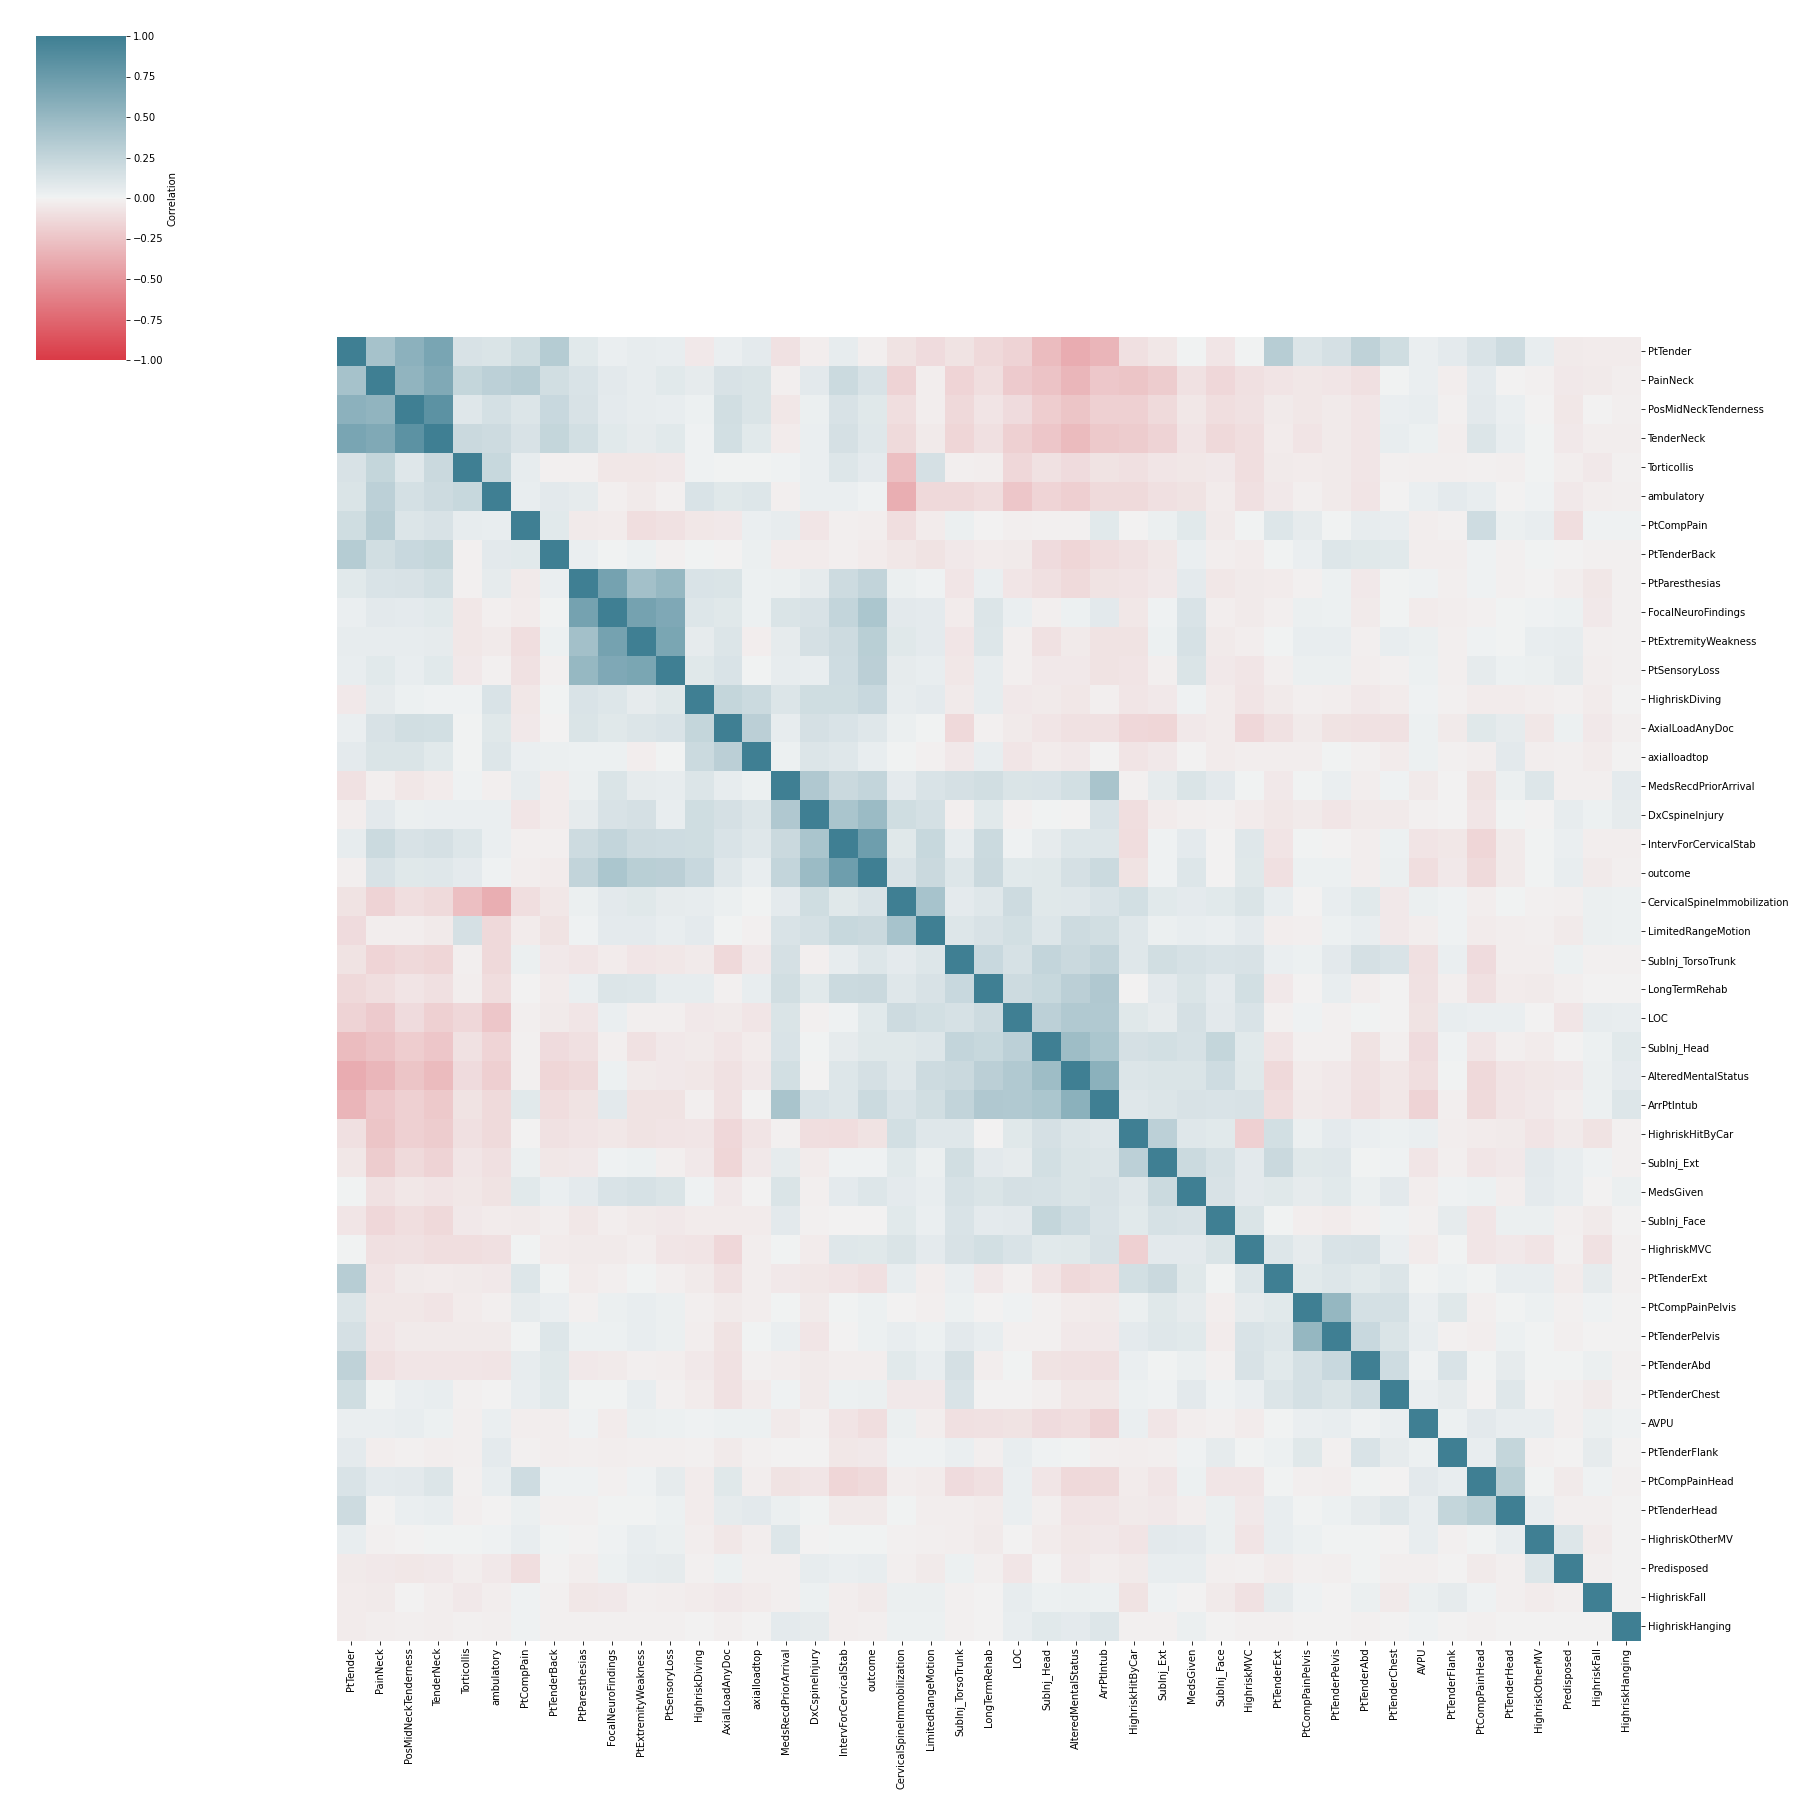
\includegraphics[height=6in, width=8in]{corr-map.png}
\centering
\caption{Correlation heatmap of reduced feature space.} 
\label{fig:corr-map}
\end{figure}

\hypertarget{sec:corr-out}{%
\subsection{Correlation with outcome}\label{sec:corr-out}}

After seeing which features are associated with each other, we then
examine the correlation of each feature with respect to the outcome
variable (whether the patient truly has a CSI). We find that most
features are not highly correlated with the outcome in either direction,
with some exceptions: the \texttt{IntervForCervicalStab} feature, which
tells whether the patient underwent any cervical stabilization measures
at the site, has the highest correlation (above 0.60) with the outcome.
This should not be surprising since a cervical stabilization measure is
only imposed on a patient if a medical official on-site thinks it is
necessary, thus we expect most true injuries to be highly associated
with this intervention.

Similarly, \texttt{DxCspineInjury} measures whether the patient is
suspected of having a CSI. This has the second-highest correlation of
roughly 0.45, which also should not be surprising. We discuss this
variable in more detail in Section \textcolor{blue}{\ref{sec:best}}.

\hypertarget{sec:modeling}{%
\section{Modeling}\label{sec:modeling}}

\hypertarget{translation}{%
\subsection{Translation}\label{translation}}

\textcolor{red}{How should one translate the question in (1) into a statistical question regarding the data to best answer the original question? Are there multiple translations? For example, can we translate the question into a prediction problem or an inference problem regarding a statistical model? List the pros and cons of each translation relative to answering the substantive question before choosing a model.}

\textcolor{red}{Do we have multiple reasonable translations?}

\hypertarget{sec:feat-sel}{%
\subsection{Feature selection}\label{sec:feat-sel}}

We use a combination of \textbf{logistic regression} and
\textbf{backwards selection} to choose our model features.

\hypertarget{sec:best}{%
\subsection{Best model}\label{sec:best}}

Our chosen model is a simple decision tree. This model achieves a
\textbf{95\% sensitivity rate} (predicting a CSI when the patient truly
has CSI) and a \textbf{70\% specificity rate} (predicting no CSI when
that is truly the case). \textcolor{red}{(I need exact values here.)}
Thus, we achieve over three times the specificity of Leonard et al.
(2011) while maintaining the same sensitivity. Statistically speaking,
we increase the power over threefold without increasing the Type I error
rate.

Prior to discovering this model, we fit a decision tree with the subset
of features obtained in Section \textcolor{blue}{\ref{sec:feat-sel}}.
This decision tree achieved a higher specificity rate of roughly 80\%.
However, this model may not be valid in a clinical context due to
certain factors that influence the reporting of a certain feature. Our
initial model has a domain-specific caveats that we must adjust for and
address.

First, the \texttt{DxCspineInjury} feature (explained in Section
\textcolor{blue}{\ref{sec:corr-out}}) has strong predictive power. This
is likely due to the fact that this predictor is literally a guess as to
whether this person has a CSI or if they arrived with a diagnosis. This
information could be revealing of the true outcome even though it is a
feature made available to a physician prior to making the CDR. A
rigorous inspection of the raw data reveals that this feature has
\textbf{zero} missing or indeterminate values. Therefore, we use this
variable can be utilized in a real-world context.

Second, some features in our data are unobservable based on the value of
other features. In the case of our initial model, the
\texttt{PtSensoryLoss} feature measures whether the patient

Subject matter expertise tells us that

\hypertarget{comparability}{%
\section{Comparability}\label{comparability}}

\textcolor{red}{Are the data units comparable or normalized so that they can be treated as if they were exchangeable? Or are apples and oranges being combined?}

\textcolor{red}{Are the data units independent? Are two columns of data duplicates of the same variable?}

\hypertarget{visualization}{%
\section{Visualization}\label{visualization}}

\textcolor{red}{Look at data or subsets of them. Create plots of 1 and 2 dimensional data. Examine summaries of such data. What are the ranges? Do they make sense? Are there any missing values? Use color and dynamic plots. Is anything unexpected? It is worth noting that 30 percent of our cortex is devoted to vision, so visualization is highly effective to discover patterns and unusual things in data. Often, to bring out patterns in big data, visualization is most useful after some model building, for example, to obtain residuals to visualize.}

\hypertarget{randomness}{%
\section{Randomness}\label{randomness}}

\textcolor{red}{Statistical inference concepts such as p-values and confidence intervals rely on randomness. What does randomness mean in the data? Make the randomness in the statistical model as explicit as possible. What domain knowledge supports such a statistical or mathematical abstraction or the randomness in a statistical model?}

\textcolor{red}{What is the randomness in this PECARN data set? Is it a random sample from a population? Which one? Why can the data be viewed as a random sample? What assumptions are being made? Can one check these conditions using the info on the data collection process?}

\hypertarget{stability}{%
\section{Stability}\label{stability}}

\textcolor{red}{What off-the-shelf method will you use? Do different methods give the same qualitative conclusion? Perturb one’s data, for example, by adding noise or subsampling if data units are exchangeable (in general, make sure the subsamples respect the underlying structures, e.g. dependence, clustering, heterogeneity, so the subsamples are representative of the original data). Do the conclusions still hold? Only trust those that pass the stability test, which is an easy-to-implement, first defense against over-fitting or too many false positive discoveries.}

\hypertarget{references}{%
\section*{References}\label{references}}
\addcontentsline{toc}{section}{References}

\hypertarget{refs}{}
\begin{CSLReferences}{1}{0}
\leavevmode\hypertarget{ref-leonard2011factors}{}%
Leonard, Julie C, Nathan Kuppermann, Cody Olsen, Lynn Babcock-Cimpello,
Kathleen Brown, Prashant Mahajan, Kathleen M Adelgais, et al. 2011.
{``Factors Associated with Cervical Spine Injury in Children After Blunt
Trauma.''} \emph{Annals of Emergency Medicine} 58 (2): 145--55.

\end{CSLReferences}

\end{document}
